\chapter{The hexagonal lattice and laminated lattices}
\scribe{Ane Santos}

\section{The hexagonal lattice}

\begin{definition}
  Let $v_1,\ldots,v_n\in \ZZ^{d}$ and the lattice $L= {}_\ZZ\!\left\langle v_1,\ldots,v_n
  \right\rangle=\left\{\sum\lambda_i v_i : \lambda_i \in \ZZ\right\}=
  \left\{M\lambda:\lambda\in \ZZ^{n}\right\}$ with
  $M=\left[v_1,\ldots,v_n\right]\in\ZZ^{d\times n}$. $M$ is called the \emph{generator
    matrix} and ${}_\ZZ\!\left\langle v_1,\ldots,v_n \right\rangle$ the \emph{integer hull} of the
  lattice.
\end{definition}


We will study two variants of the hexagonal lattice:
\[
  A_{2,\RR^{2}}
  \ = \
  \left\{\begin{bmatrix}
        1 & 1/2 \\
        0 & \sqrt{3}/2 \end{bmatrix}\lambda:\lambda\in\ZZ^{2}\right\}, 
    \qquad
  A_{2,\RR^{3}}
  \ = \
  \left\{\begin{bmatrix}
        1 & 0 \\
        -1 & 1 \\
        0 & -1 \end{bmatrix}\lambda:\lambda\in\ZZ^{2}\right\},
\]
with respective generating matrices
$M=\left[\begin{smallmatrix}
      1 & 1/2 \\
      0 & \sqrt{3}/2 \end{smallmatrix}\right]$ and
$M'=\left[\begin{smallmatrix}
      1 & 0 \\
      -1 & 1 \\
      0 & -1 \end{smallmatrix}\right]$. 

Firstly, we study $A_{2,\RR^{3}}$:

\begin{figure}[htbp]
\centering
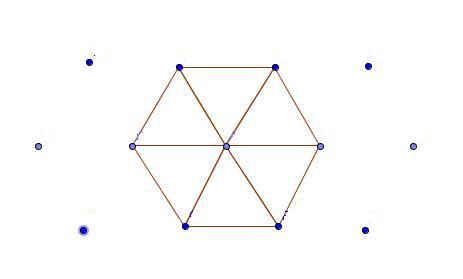
\includegraphics[width=0.5\textwidth]{apunteaklattice}
\caption{$A_{2,\RR^{3}}$}
\end{figure}


\begin{displaymath}
	A_{2,\RR^{3}}=\left\{M'\lambda:\lambda\in\ZZ^{2}\right\}=\left\{\begin{bmatrix}
	\lambda_1 \\
	-\lambda_1 + \lambda_2 \\
	-\lambda_2 \end{bmatrix}:\lambda_1,\lambda_2\in\ZZ\right\}
\end{displaymath}

We want to find a hyperplane that contains $A_{2,\RR^{3}}$. We are in $\RR^{3}$, so this
hyperplane is of the form $\left\{x\in\RR^{3}:\left\langle
    a,x\right\rangle=a_0\right\}$. But we know $0$ is in $A_{2,\RR^{3}}$ so $a_0=0$ and
\[
  H \ = \ 
  \left\{x\in\RR^{3}:\left\langle a,x\right\rangle=0\right\} 
  \ = \ 
  \left\{\omega\in\RR^{3}:\left\langle \omega,x\right\rangle, \forall \in \colspan
    M\right\},
\]
 where $\colspan
M={}_\RR\!\left\langle v_1,\ldots,v_n \right\rangle=\im M$ (it is an abelian group and it is
also a vector space). So, $H=\left\{x\in\RR^{3}: \left\langle
    a,x\right\rangle=0\right\}=\ker M$

$\dim \im M=2$ and $\dim A_{2,\RR^{3}}=3$ $\Longrightarrow$ $\dim A_{2,\RR^{3}}=\dim \ker M +\dim \im M$ $\Longrightarrow$ $\dim \ker M=1$

A generator of $\ker M$ will be $\left(\begin{smallmatrix}
1 \\
1 \\
1 \end{smallmatrix}\right)$

$\left[1 1 1\right]\left[\begin{smallmatrix}
1 & 0 \\
-1 & 1 \\
0 & -1 \end{smallmatrix}\right]=\left[0 0\right]$ $\Rightarrow$ $\ker M= {}_\RR\!\left\langle \left[1 1 1\right]\right\rangle$

So $A_{2,\RR^{3}}\subset\left\{x\in\RR^{3}: x_1+x_2+x_3=0\right\}=\left\{x\in\RR^{3}: \mathbbm{1}x=0\right\}$


\begin{definition}
The \emph{Gram matrix} of a lattice $L$ with generator matrix $M$ is $G_L=M^{T}M$.
\end{definition}


\begin{definition}
The \emph{determinant of a lattice} $L$ with generator matrix $M$ is the determinant of the Gram matrix.
$\det L=\det M^{T}\cdot \det M=\left(\det M\right)^{2} $
\end{definition}


\begin{observation}
 $G_L$ is always a symmetric matrix because $G_L^{T}=\left(M^{T}M\right)^{T}=M^{T}M$.
\end{observation}


We calculate the determinants of $A_{2,\RR^{2}}$ and $A_{2,\RR^{3}}$:

\begin{eqnarray*}
  \det A_{2,\RR^{2}}
  &=&
  \det \begin{bmatrix}
      1 & 0 \\
      \tfrac12 & \tfrac12\sqrt{3} \end{bmatrix}\cdot\begin{bmatrix}
      1 & \tfrac12 \\
      0 & \tfrac12\sqrt{3} \end{bmatrix}
    \ = \ 
    (\tfrac12\sqrt{3})(\tfrac12\sqrt{3})
  \ = \ 
  \frac34,
  \\
  \det A_{2,\RR^{3}}
  &=&
  \det \begin{bmatrix}
      0 & -1 & 0 \\
      0 & 1 & -1\end{bmatrix}\cdot\begin{bmatrix}
      1 & 0 \\
      -1 & 1 \\
      0 & -1 \end{bmatrix}=\det \begin{bmatrix}
      2 & -1 \\
      -1 & 2 \end{bmatrix}
  \ = \
  3.
\end{eqnarray*}

\begin{definition}
The \emph{minimum norm} of a lattice $L$ is $\mu_L=\min\left\{\left\|v\right\|^{2}:v\in L\backslash \left\{0\right\}\right\}$
\end{definition}

From the minimum norms $\mu_{A_{2,\RR^{2}}} = 1$, $\mu_{A_{2,\RR^{3}}} = \sqrt{2}$, we
conclude that both the determinants and the minimum norms of $A_{2,\RR^{2}}$ and
$A_{2,\RR^{3}}$ are different. However, we should not conclude that these lattices are
really different:


\begin{definition}
Two lattices are \emph{isomorphic} if one is obtained from the other by rotation, reflection, translation and scaling.
\end{definition}

The most general map between isomorphic lattices is therefore of the form
\[
   x\ \longmapsto \ \alpha A+t, \qquad\text{where }
   t\in\RR^{n},\; A\in O(n),\; \alpha\in\RR^{*}.
\]
Note that negative $\alpha$ correspond to reflections.

\begin{definition}[Packing density of L]
  $\Delta_L=\frac{\vol(\text{sphere in packing})}{\vol(\Pi_L)=\sqrt{detL}}$,
  where $\Pi_L=\left\{\sum\lambda_i v_i : \lambda_i\in\left[0,1\right)\right\}$ is the
  fundamental parallelopiped.
\end{definition}

To calculate the packing density of $A_{2,\RR^{2}}$ and $A_{2,\RR^{3}}$, note that in
$A_{2,\RR^{2}}$ the radius of the sphere is~$\frac{1}{2}$ so the volume is
$\left(\frac{1}{2}\right)^{2}\pi$. We obtain the same density, which is as it should be
for isomorphic lattices:
\begin{eqnarray*}
  \Delta_{A_{2,\RR^{2}}}
 &=&
  \frac{\left(\frac{1}{2}\right)^{2}\pi}{\sqrt{3/4}}
  \ = \
  \frac{\pi}{2\sqrt{3}},
 \\
  \Delta_{A_{2,\RR^{3}}}
 &=&
  \frac{\left(\frac{1}{2}\sqrt{2}\right)^{2}\pi}{\sqrt{3}}
  \ = \
  \frac{\pi}{2\sqrt{3}}.
\end{eqnarray*}

The connection between these two representations is via the map
\[
 \begin{bmatrix}
1 & \frac{-1}{\sqrt{3}} \\
-1 & \sqrt{3} \\
0 & \frac{-2}{\sqrt{3}}\end{bmatrix}
\begin{bmatrix}
1 & \frac{1}{2} \\
0 & \frac{\sqrt{3}}{2}
\end{bmatrix}
\ = \
\begin{bmatrix}
1 & 0 \\
-1 & 1 \\
0 & 1\end{bmatrix}.
\]

So, we have two different ways to write the same lattice. The advantages of $M'$ over $M$
are that the coordinates are nicer and the symmetries of the lattice are more easily seen.


\begin{claim}
Any permutation of the coordinate axes in $\RR^{3}$ is a symmetry of $A_{2,\RR^{3}}$.
\end{claim}


\begin{proof}
  Let $P:\RR^{2}\longrightarrow\RR^{3}$ be a symmetry of $L=A_{2,\RR^{3}}$, so that
  $P(L)=L$. This means that for all $x\in L$, we should have $P(x)\in L$, which is in turn
  equivalent to the condition that for all $\lambda\in\ZZ^{2}$, there must exist
  $\beta\in\ZZ^{2}$ such that
  \begin{equation}\label{eq:beta}
    M\beta
    \ = \
    PM\lambda.
  \end{equation}
  (In particular, this coordinatizes $x\in L$ as $x=M\lambda$).

  We want to prove that if $P$ is a permutation, then for any $\lambda\in\ZZ^{2}$ we can
  always find a~$\beta\in\ZZ^2$ that makes equation~\eqref{eq:beta} true.  We know $P$,
  $M$ and $\lambda$, so we have to find $\beta$. This is a linear equation for~$\beta$.
  We must show that the linear equation $M\beta=b$ has a unique solution for any
  $b=b_\lambda =PM\lambda$.  The solution is unique if $\rank M$ is maximal, i.e. $\rank
  M=2$. By inspection, $M$~really has rank 2, so we only have to see if it always has a
  solution.  From the Fundamental Theorem of Linear Algebra (part 2)
  \cite{strang-linear-algebra},~\cite{strang-ftla}, the
  system~\eqref{eq:beta} has a solution if and only if
\begin{eqnarray*}
  && b\in \colspan M=\im M 
  \\ &\Longleftrightarrow&
  b\bot\left(\colspan M\right)^{\bot}
  \\ &\Longleftrightarrow&
  b^{T}y=0 \text{ whenever } y\bot \colspan M 
  \\ &\Longleftrightarrow&
  b^{T}y=0 \text{ whenever } y^{T}M=0.
\end{eqnarray*}
Since  $\left[y_1 y_2 y_3\right]\left[\begin{smallmatrix}
1 & 0 \\
-1 & 1 \\
0 & -1\end{smallmatrix}\right]=\left[y_1 - y_2, y_2 - y_3\right]$, we conclude that
$y^{T}M=0$ if and only if
\[
0 y=\alpha\mathbbm{1}
b^{T}y=\lambda^{T}M^{T}P^{T}\alpha\mathbbm{1}=\alpha\lambda^{T}M^{T}P^{T}\mathbbm{1}=\alpha\lambda^{T}M^{T}\mathbbm{1};
\]
but $M^{T}\mathbbm{1}=0$ because $\mathbbm{1}$ is in the $\ker$ of $M$.
\end{proof}


\section{Laminated lattices}


Define $\mathbb{L}_0=\left\{L^{0}\right\}$, $L^{0}=\left\{0\right\}=\mathbb{R}^{0}$ the
zero dimensional lattice and $m:=4$ (usually $m$ is 4 because then the spheres in the
corresponding lattice packing have radius 1).

For $n>0$, $\mathbb{L}_{n+1}=\left\{L_1^{n+1},\ldots,L_{a_n}^{n+1}\right\}$ is the collection of $n+1$-dimensional lattices such that
\begin{enumerate}
\item each $L_i^{n+1}$ has constant minimal norm $m$
\item each $L_i^{n+1}$ contains at least one $L_j^n$ as a sublattice
\item each $L_i^{n+1}$ has minimal determinant subject to (1), (2)
\end{enumerate}


We will see which are these lattices:

\begin{description}
\item[$\mathbb{L}_1$] This lattice must be of the form  $k\ZZ$.
It needs minimal norm $m=4$, so we must take $2\ZZ$, which satisfies (2) and (3).
So the unique laminated lattice of rank~1 is $2\ZZ$.


\item[$\mathbb{L}_2$] Taking $M=\left[\begin{smallmatrix}
      2 & 0 \\
      0 & 2\end{smallmatrix}\right]$ satisfies (1),(2) and (3), and yields
  $2\ZZ^{2}$. However, it is not necessary that our laminated lattice contain only integer
  points, the only condition is that it must contain~$2\ZZ$. Thus, we have the two
  candidates $2\ZZ^{2}$ and $A^{2}$. We decide between the two by
  calculating the determinant corresponding to the generator matrices $M_1=
  \left[\begin{smallmatrix}
    4 & 0\\
    0 & 4
  \end{smallmatrix}\right]$ and $M_2 = \left[\begin{smallmatrix}
        2 & 1 \\
        0 & \sqrt{3} \end{smallmatrix}\right]$:
  \begin{eqnarray*}
    \det 2\ZZ^{2} 
    & = & 
    \det M_1^{T}M_1 \ = \ \det\begin{bmatrix}
        4 & 0 \\
        0 & 4 \end{bmatrix} \ = \ 16;
      \\
    \det A_2
    &=& 
    \det M_2^{T}M_2 \ = \ \det\begin{bmatrix}
        4 & 2 \\
        2 & 4 \end{bmatrix} \ = \ 12.
\end{eqnarray*}
We see that $\det A_2 < \det 2\ZZ^{2}$, which comes about because the area of the
fundamental parallelopiped for $A_2$ is less than that of the square. So $\mathbb{L}_2$
is~$A_2$.
\end{description}
We will see now how can we do the sphere packing:

\begin{figure}[htbp]
\centering
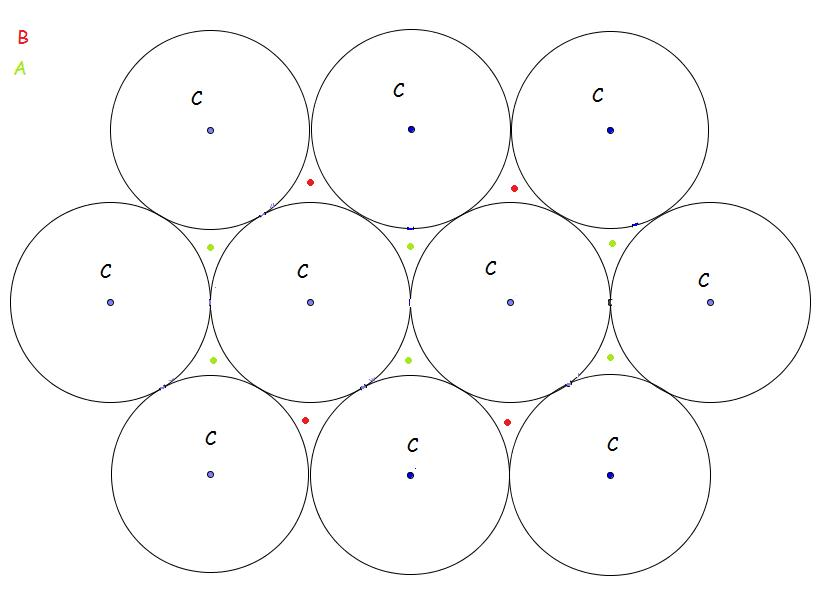
\includegraphics[width=0.5\textwidth]{apunteslattice}
\caption{sphere packing}
\end{figure}

For the next layer we have two options, put them (the centers of the sphere) over the deep holes A or over the deep holes B. For the second layer we put, we will have the possibility of putting them over C (the centers of the spheres of the first layer).
Each lattice obtained by snugly packing copies of $A_2$ is determied by the sequences
ABAB.... (this is the hexagonal close packing(He attoms))
ABCABC....(this is the face-centered cubic lattice ($A_3$))
of equivalence classes of deep holes.

In each step there are two options to choose from, which makes uncountably many possibilities in total.



% Local Variables: 
% mode: latex
% TeX-master: "dag-upc"
% End: 
